% !TeX spellcheck = ru_RU_yo
% !TEX program = xelatex

\documentclass[pta]{../../../scs-iam}

\begin{document}

\newgeometry{
  top=20mm,
  right=15mm,
  bottom=20mm,
  left=20mm,
  bindingoffset=0cm
}

\thispagestyle{empty}

\begin{center}
  {
    \bfseries
    {
      \subnormal
      Министерство образования и науки Российской Федерации
    } \\[-0.5em]
    {
      \scriptsize
      ФЕДЕРАЛЬНОЕ ГОСУДАРСТВЕННОЕ АВТОНОМНОЕ ОБРАЗОВАТЕЛЬНОЕ УЧРЕЖДЕНИЕ ВЫСШЕГО ОБРАЗОВАНИЯ
    } \\[-0.25em]
    {
      \subnormal
      “САНКТ-ПЕТЕРБУРГСКИЙ НАЦИОНАЛЬНЫЙ ИССЛЕДОВАТЕЛЬСКИЙ \\[-0.5em]
      УНИВЕРСИТЕТ ИНФОРМАЦИОННЫХ ТЕХНОЛОГИЙ, \\[-0.75em]
      МЕХАНИКИ И ОПТИКИ”
    } \\[1em]
  }
\end{center}

\small

\begin{center}
  {
    \normalsize
    \textbf{Д Н Е В Н И К\quad П Р А К Т И К И}
  } \\[-0.25em]
  за период с \underline{\makebox[.2\textwidth][c]{30.04.2018}} по \underline{\makebox[.2\textwidth][c]{03.06.2018}}
\end{center}

{
  \parindent 0pt

  \textbf{Студент}
  $\underset{
    \text{\scriptsize (Фамилия, Имя, Отчество)}
  }{
    \underline{\makebox[.65\textwidth][l]{Кузнецов Андрей Андреевич}}
  }$
  \hfill
  \textbf{Группа №}
  \underline{\makebox[.1\textwidth][c]{\strut P4215~~}} \\[-1em]
  
  \textbf{Факультет}
  \uline{программной инженерии и компьютерной техники \hfill} \\[-1em]

  \textbf{Кафедра}
  \uline{информатики и прикладной математики \hfill} \\[-1em]

  \textbf{Направление подготовки (специальность)}
  \uline{09.04.01 \hfill} \\[-1em]

  \textbf{Место прохождения практики}
  \uline{ИП Николаев Денис Александрович \hfill} \\[-1em]
  
  \titledline{\textbf{Руководитель практики от организации}}
  $\underset{
    \text{\scriptsize (Фамилия И.О., должность и место работы)}
  }{
    \underline{\makebox[\remaining][s]{Фёдоров Е.М., ИП Николаев Д.А., руководитель от-}}
  }$
  \uline{дела разработки программного обеспечения\hfill} \\[-1em]
  
  \titledline{\textbf{Руководитель практики от университета}}
  $\underset{
    \text{\scriptsize (Фамилия И.О., должность)}
  }{
    \underline{\makebox[\remaining][l]{Исаев И.В., ассистент}}
  }$ \\[1.5em]

  \begin{flushright}
    \begin{minipage}{.5\textwidth}
      Индивидуальное задание выполнено полностью \\
      $\underset{
        \text{\scriptsize (подпись ответственного за проведение практики от университета)}
      }{
        \underline{\makebox[\textwidth][s]{\strut}}
      }$ \\[1em]

      \datetemplate
    \end{minipage}
  \end{flushright}
}

\vfill

\begin{center}
  {
    \normalsize
    Санкт-Петербург \\
    2018 г.
  }
\end{center}

\restoregeometry
\normalsize

\clearpage

\setcounter{page}{2}

{
  \parindent 0pt

  \begin{center}
    \begin{figure}[h!]
      \centering
      \setlength{\fboxsep}{0pt}
      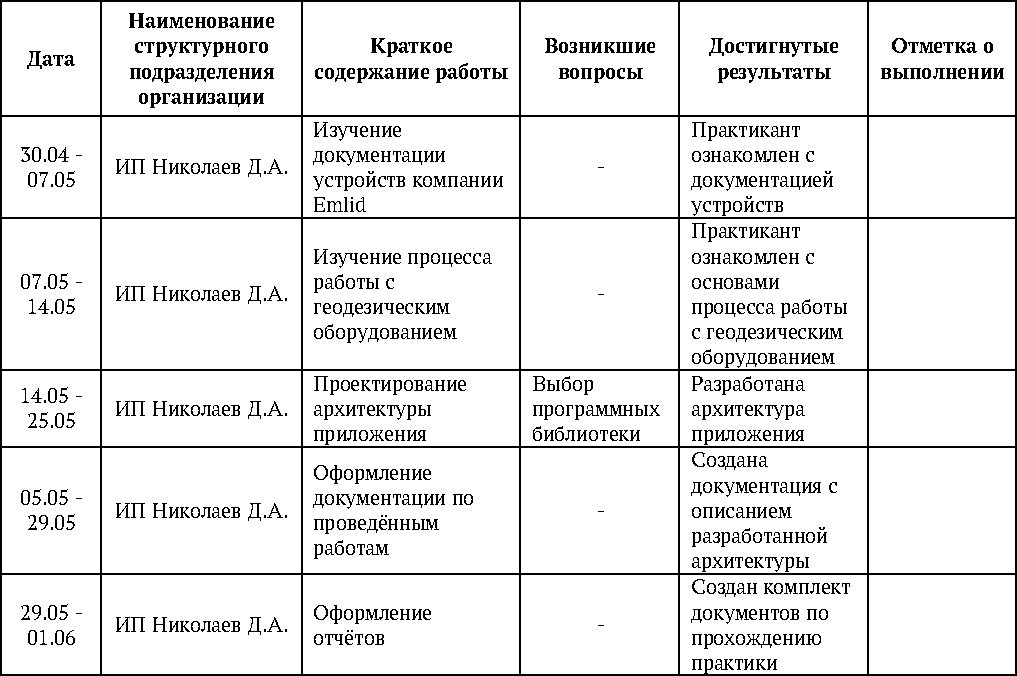
\includegraphics[width=\textwidth]{table}
    \end{figure}
  \end{center}
}

\end{document}
